\documentclass[12pt,AutoFakeBold]{article} 
\usepackage[专业实验实践能力(B级)达标测试]{XDUreport}  % 科目名称
\problem{雾霾探测系统设计}  % 请在此处填写问题内容
\labdate{2022 年 05 月 07 日}
% 其他参数在宏包中进行更改,其中学院,班级,姓名,学号均在sty宏包内进行更改
% \usepackage{fourier}  % 这是 fourier 字体,更柔和 

%% 如果你需要中文的一级标题编号,如“一、”、“二、”等,请把下面两行取消注释
% \RequirePackage{zhnumber} % change section number to chinese
% \titleformat{\section}{\Large\bfseries\rmfamily}{\zhnum{section}、}{0em}{}

% 文档开始
        
\begin{document}

\maketitle
\setcounter{tocdepth}{2}

\tableofcontents  % 生成目录

% 正文标题
\makeatletter
\begin{center}
    \LARGE \textbf{\textsf{\@problem}}
\end{center}
\makeatother

% 正文开始

\section{任务描述}

雾霾的频繁出现已严重的影响到人们的出行,对人们的健康造成了重大影响。因此,能在出行前查看雾霾的指数,并采取相应的措施来把雾霾的影响降到最小就显得尤为重要。本系统在分析多种因子的影响下,设计一款手机端雾霾 app 探测系统。要求如下:

\begin{enumerate}[1.]
\item 定位功能:将定位城市保存在服务器端,并同时显示在客户端。
\item 界面设计:包含显示天气和空气质量指数的动态显示。
\item 天气详情和空气质量指数:定位后的城市在服务器端获取后,传给天气详情界面,通过所传城市用百度天气api获取对应的天气详情和空气质量指数,并保存在服务器端。
\item 完成报告。
\end{enumerate}

\section{方案设计与论证}

\subsection{系统方案}

我计划用 Python Flask 框架设计网页版雾霾探测系统,static 文件夹用于存放包括 css 样式、背景图像和 javascript 脚本在内的各种静态文件,templates 文件夹用于存放网页主体 html 文件,用 flask 框架的 render\_template 函数渲染 html 文件,运行 app.py 文件可在本地默认的 127.0.0.1:5000 查看渲染结果,可以手动更改 host 和 port。

整个 html 文件主体是两个部分,第一个部分包括时间、地理、天气和空气质量信息的获取与展示,考虑使用 jQuery 的幻灯片插件 OWL Carousel 对这一部分进行模板渲染;第二部分是未来一周的气温和天气预测,考虑用 echarts 绘制动态折线图进行展示,这一部分官网有现成的天气折线模板代码 \url{https://echarts.apache.org/examples/zh/editor.html?c=line-marker},只需稍作修改加入即可。

\subsection{系统实现}

首先考虑如何获取位置信息,由于百度、高德地图等浏览器端的 js 定位接口需要支持 https 不是那么方便,故我选择使用 ip 定位,ip 定位精确度高,而且大部分天气数据 api 也支持 ip 来查询,本项目中我使用的 ip 查询接口为 \url{http://ip-api.com/json/},获取 ip 得到 json 的文件如图 \ref{fig:ipjson} 所示,我用到了其中的城市和经纬度信息用于后续信息查询。

\begin{figure}[htbp]
	\centering
	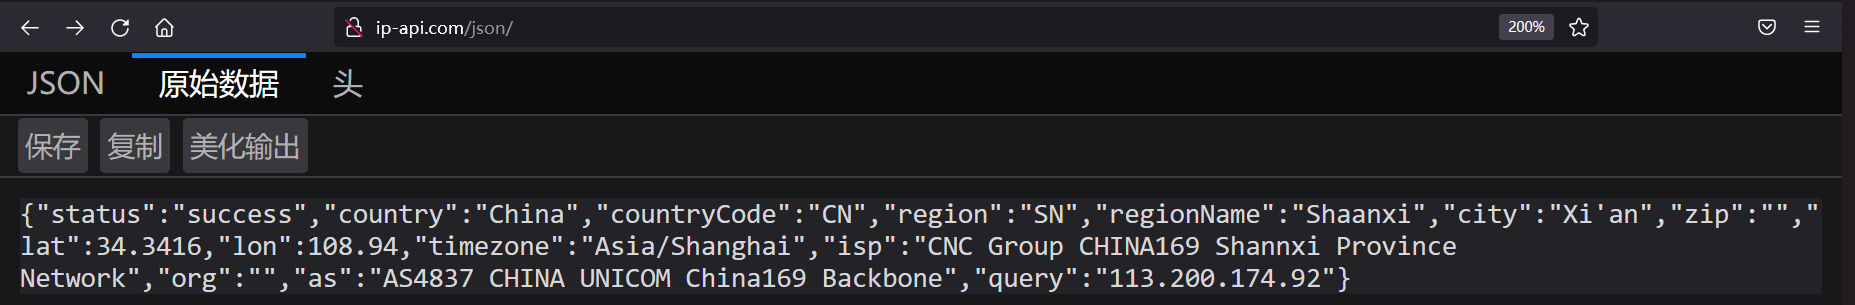
\includegraphics[width=\textwidth]{ipjson.png}
	\caption{获取 ip 得到的 json 文件} \label{fig:ipjson}
\end{figure}

时间获取较为简单,可以直接用 js 内置函数获取,这里略去。接下来考虑获取天气和空气质量信息,可以用和风天气开发平台方便的获取到,天气信息获取官方文档见 \url{https://dev.qweather.com/docs/api/weather/weather-now/},注册账号获取 KEY 后,利用经纬度信息查询到天气信息和空气信息 json 文件分别如图 \ref{fig:weatherjson} 和图 \ref{fig:airjson} 所示,

\begin{figure}[htbp]
	\centering
	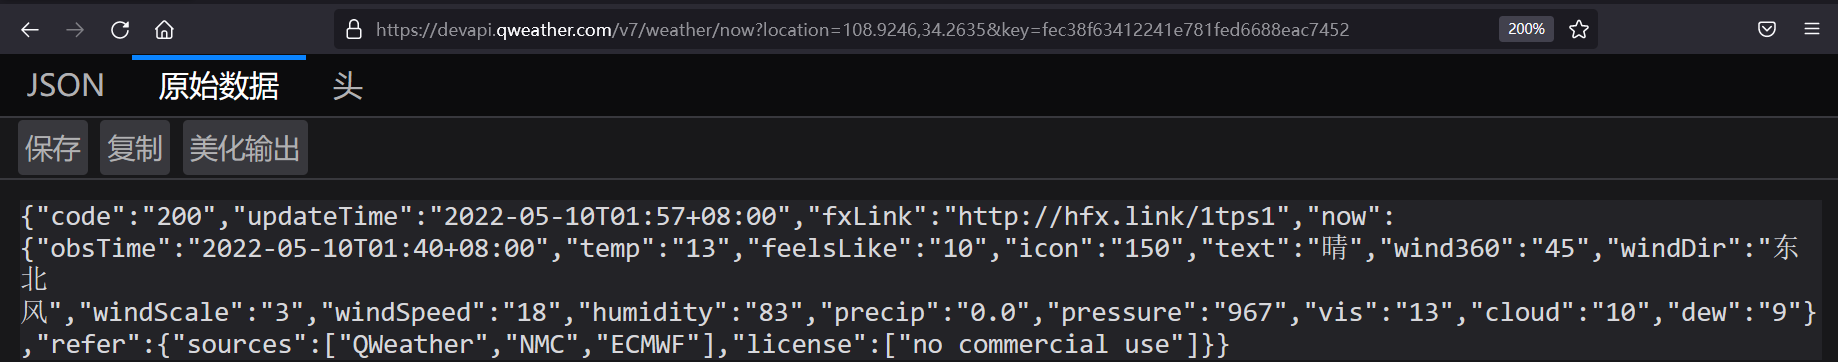
\includegraphics[width=\textwidth]{weatherjson.png}
	\caption{天气信息 json 文件} \label{fig:weatherjson}
\end{figure}

\begin{figure}[htbp]
	\centering
	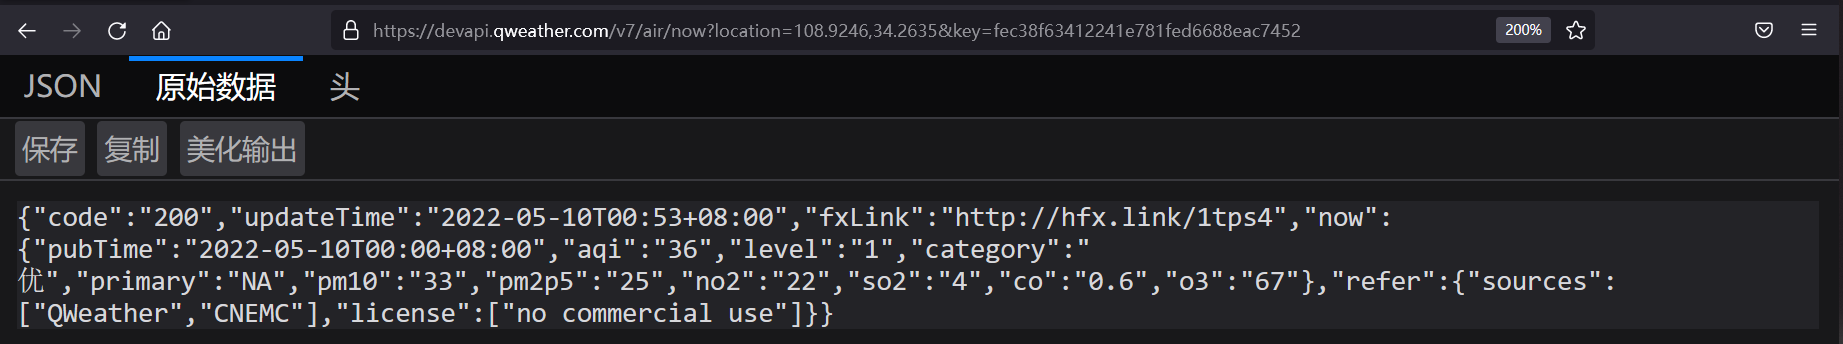
\includegraphics[width=\textwidth]{airjson.png}
	\caption{空气信息 json 文件} \label{fig:airjson}
\end{figure}

关于第二部分一周天气预测信息获取考虑使用天气 API,官方文档见 \url{https://www.tianqiapi.com/index/doc?version=week},获取账号和密钥后可通过城市 id、名称或 ip 查询天气信息,优先级递减,默认返回当前 ip 城市天气,我的项目中只使用 json 文件中的日期、气温和天气信息绘制折线图。这一部分直接参考 echarts 官网折线代码模板稍作修改填充信息即可。

包括 css 样式和 js 脚本在内的其他文件,只需调好颜色、字体和布局即可,不属于报告的主要部分,这里略去。

\section{结果与展示}

第一部分界面如图 \ref{fig:main1} 所示,其中 4 个栏目信息如图 \ref{fig:subfig} 所示。

\begin{figure}[htbp]
	\centering
	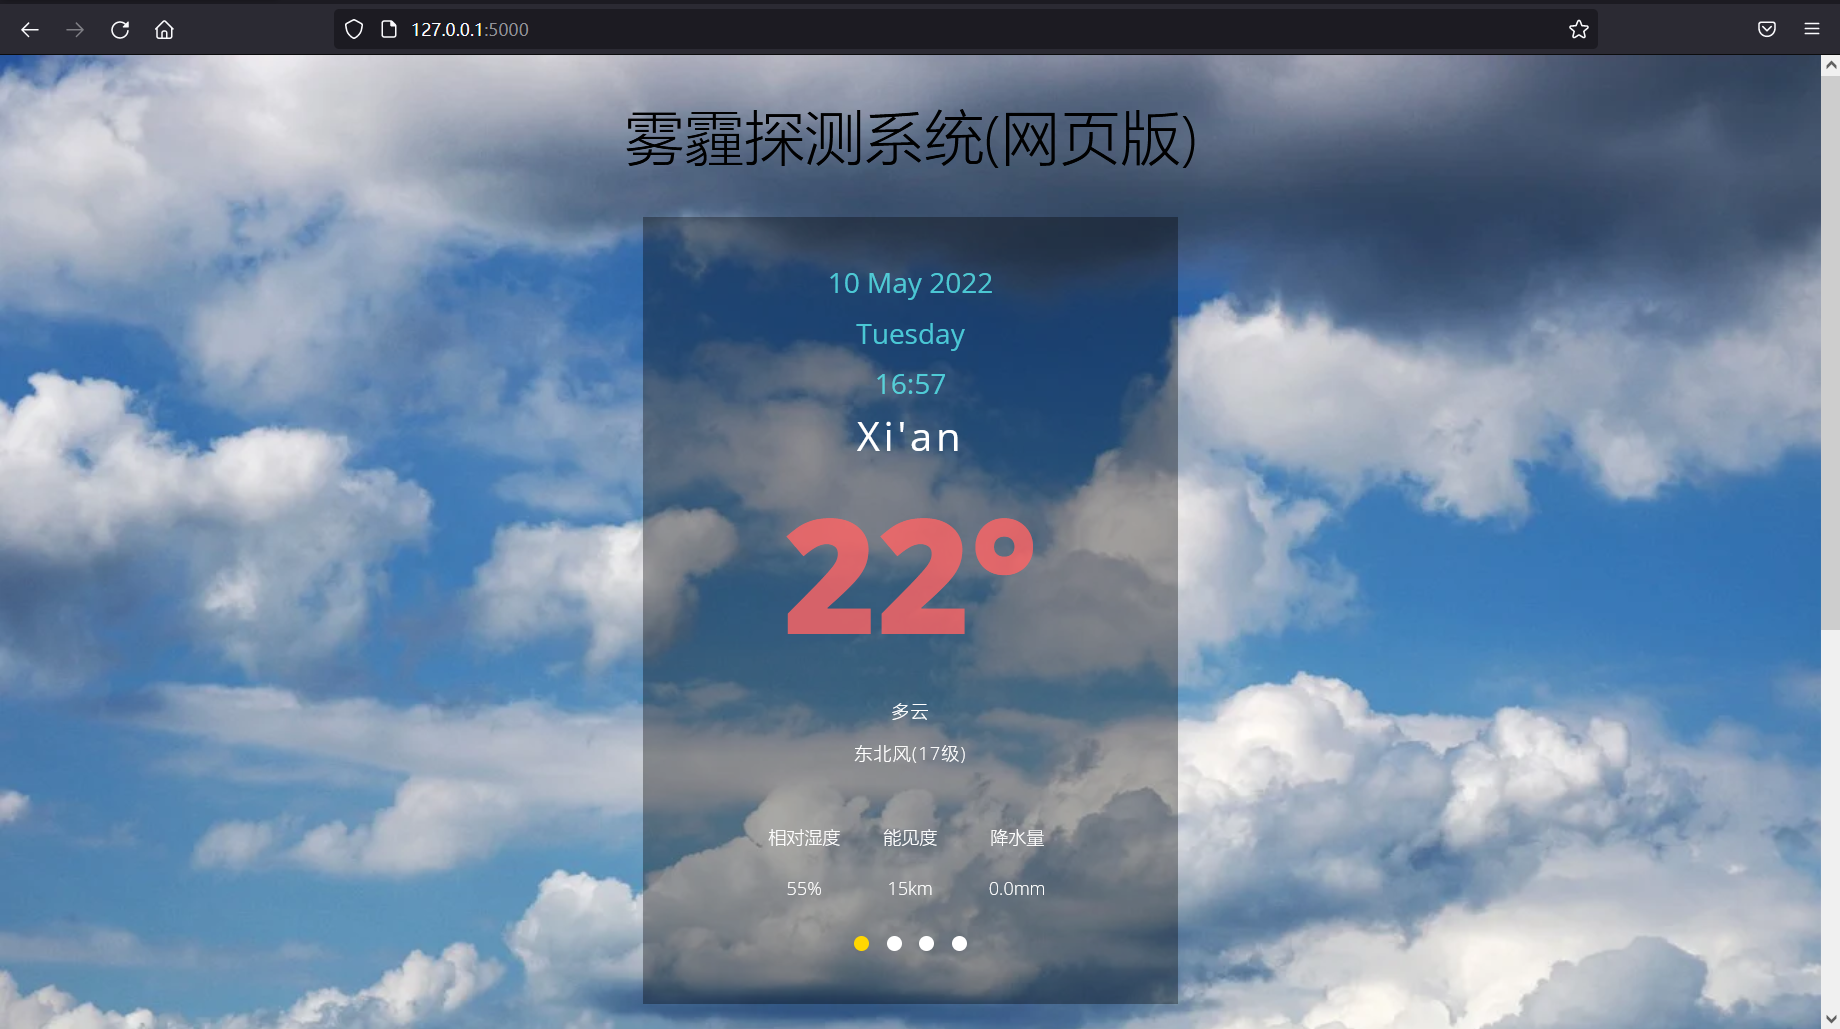
\includegraphics[width=\textwidth]{main1.png}
	\caption{第一部分界面展示} \label{fig:main1}
\end{figure}

\begin{figure} 
\centering 
\subfigure[第一部分栏目 1 信息]{\label{fig:subfig:a}
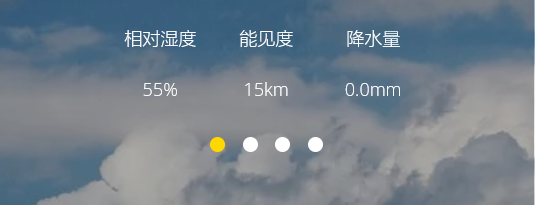
\includegraphics[width=0.45\linewidth]{item1.png}}
\hspace{0.01\linewidth}
\subfigure[第一部分栏目 2 信息]{\label{fig:subfig:b}
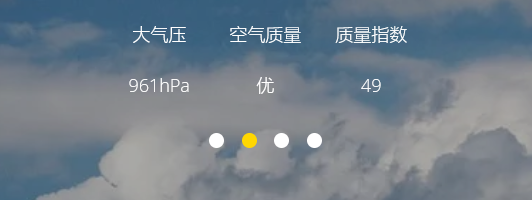
\includegraphics[width=0.45\linewidth]{item2.png}}
\vfill
\subfigure[第一部分栏目 3 信息]{\label{fig:subfig:a}
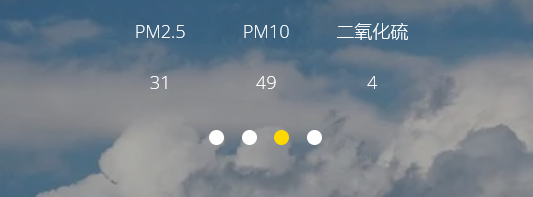
\includegraphics[width=0.45\linewidth]{item3.png}}
\hspace{0.01\linewidth}
\subfigure[第一部分栏目 4 信息]{\label{fig:subfig:b}
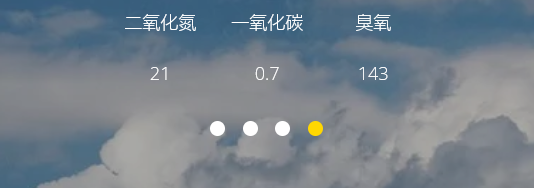
\includegraphics[width=0.45\linewidth]{item4.png}}
\caption{第一部分栏目信息展示}
\label{fig:subfig}
\end{figure}

第二部分界面如图 \ref{fig:main2} 所示。

\begin{figure}[htbp]
	\centering
	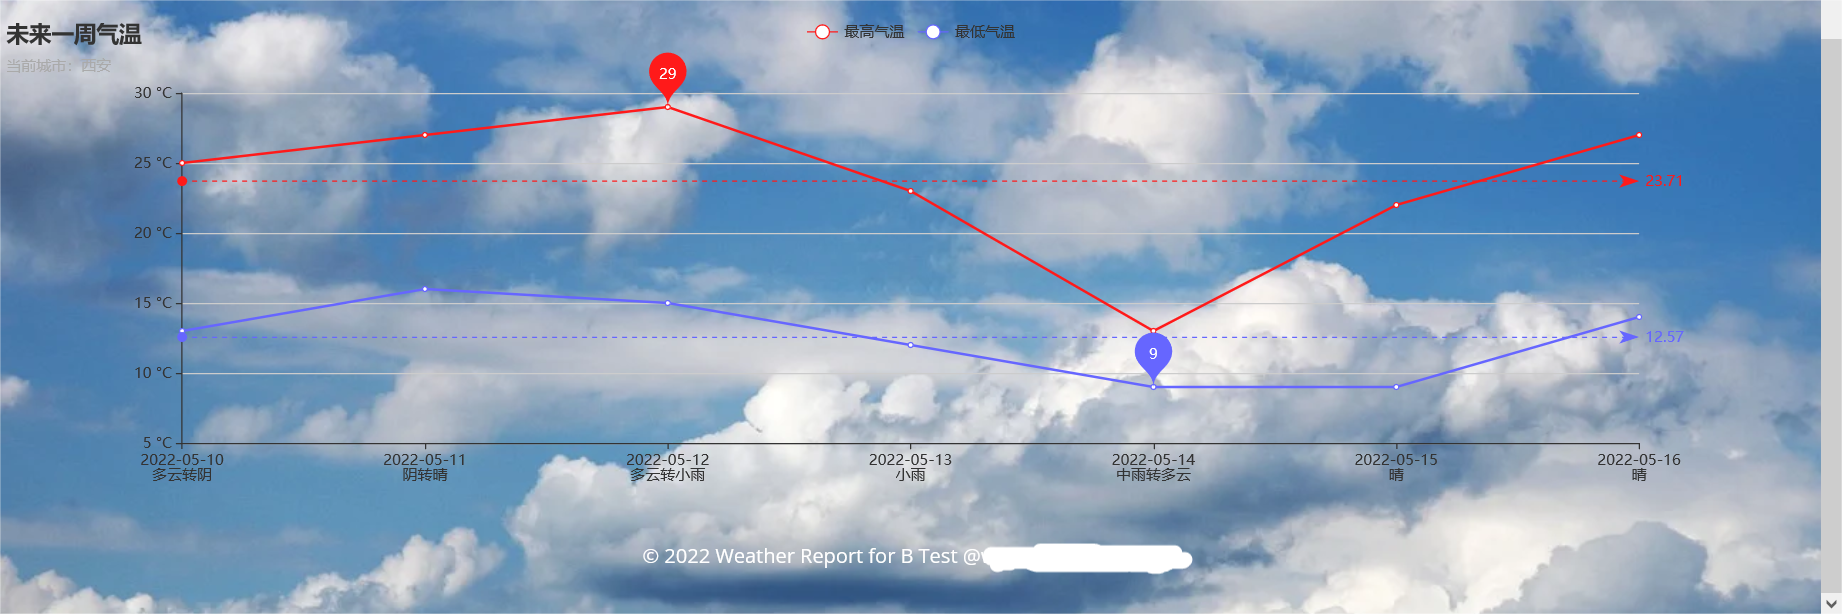
\includegraphics[width=\textwidth]{main2.png}
	\caption{第二部分界面展示} \label{fig:main2}
\end{figure}

\section{总结}

通过本次项目实践,可以独自完成基础的 web 开发,整个项目由本人一人完成,我认为本次项目完成的较为完整美观且功能齐全,但不足是时间相关代码没有优化,需要手动刷新页面更新时间。项目主要代码放在附录,css 样式和 js 脚本等不是主要部分略去。

\newpage
\begin{appendices} 

\section{项目主要代码}

\subsection{app.py}

\begin{lstlisting}[language=python]
from flask import Flask
from flask import render_template
from gevent.pywsgi import WSGIServer

app = Flask(__name__)

@app.route('/')
def info_handler():
    return render_template('index.html')

if __name__ == '__main__':
    # from waitress import serve
    # serve(app, host="127.0.0.1", port=5000)
    app.run()
    # http_server = WSGIServer(('', 4000), app)
    # http_server.serve_forever()
\end{lstlisting}

\subsection{第一部分}

\begin{lstlisting}[language=html]
	<div class="main-agileits">
        <h1><b>雾霾探测系统(网页版)</b></h1>
		<div class="main-wthree-row"> 
			<div class="agileinfo-text"> 
				<div class="date">
				    <script type="text/javascript">
						var mydate=new Date()
						var year=mydate.getYear()
						if(year<1000)
						year+=1900
						var day=mydate.getDay()
						var month=mydate.getMonth()
						var daym=mydate.getDate()
						if(daym<10)
						daym="0"+daym
						var dayarray=new Array("Sunday","Monday","Tuesday","Wednesday","Thursday","Friday","Saturday")
						var montharray=new Array("January","February","March","April","May","June","July","August","September","October","November","December")
						var h=mydate.getHours()
                        var m=mydate.getMinutes()
                        var s=mydate.getSeconds()
                        if (m<10) m="0"+m
                        if (s<10) s="0"+s
                        document.write(daym+"  "+montharray[month]+"  "+year+" <br> "+dayarray[day] + " <br> " +h+":"+m)
                    </script>
				</div>
                <h4 class="location"></h4>
				<h2 class="temp">&nbsp;</h2>
				<h6 class="weather"></h6>
                <h6 class="wind"></h6>
			</div>
			<div class="w3layouts-slider">
				<div id="owl-demo" class="owl-carousel owl-theme">
                    <div class="item agile-item">
						<h6>相对湿度</h6>
                        <br>
						<h6 class="humidity"></h6>
					</div> 
                    <div class="item agile-item">
						<h6>能见度</h6>
                        <br>
						<h6 class="vis"></h6>
					</div> 
                    <div class="item agile-item">
						<h6>降水量</h6>
                        <br>
						<h6 class="precip"></h6>
					</div> 
                    <div class="item agile-item">
						<h6>大气压</h6>
                        <br>
						<h6 class="pressure"></h6>
					</div> 
					<div class="item agile-item">
						<h6>空气质量</h6>
                        <br>
						<h6 class="quality"></h6>
					</div> 
					<div class="item agile-item">
						<h6>质量指数</h6>
                        <br>
						<h6 class="aq"></h6>
					</div> 
					<div class="item agile-item">
                        <h6>PM2.5</h6>
                        <br>
						<h6 class="pm25"></h6>
					</div>  
                    <div class="item agile-item">
                        <h6>PM10</h6>
                        <br>
						<h6 class="pm10"></h6>
					</div>  
					<div class="item agile-item">
                        <h6>二氧化硫</h6>
                        <br>
						<h6 class="so2"></h6>
					</div> 
					<div class="item agile-item">
                        <h6>二氧化氮</h6>
                        <br>
						<h6 class="no2"></h6>
					</div> 
					<div class="item agile-item">
                        <h6>一氧化碳</h6>
                        <br>
						<h6 class="co"></h6>
					</div>  
					<div class="item agile-item">
                        <h6>臭氧</h6>
                        <br>
						<h6 class="o3"></h6>
					</div> 
				</div>
				<script>
					 var icons = new Skycons({"color": "#fff"}),
						  list  = [
							"clear-night","clear-day", "partly-cloudy-day",
							"partly-cloudy-night", "cloudy", "rain", "sleet", "snow", "wind",
							"fog"
						  ],
						  i;
					  for(i = list.length; i--; )
						icons.set(list[i], list[i]);
					  icons.play();
				</script>
			</div>
	</div>
\end{lstlisting}

\subsection{第二部分}

\begin{lstlisting}[language=html]
	<div id="weather" class="col-lg-12 col-md-12" style="height:400px"></div>
            <div class="get_weather_info">
                <script>
                    $.get("http://ip-api.com/json/", function(basic){
                        // 旧版本 https://free-api.heweather.net/s6/weather/now?location=" + basic['ip'] + "&key=b27e0f8b9678447c91a8edbcded8b055
                        $.get("https://devapi.qweather.com/v7/weather/now?location=" + basic['lon'] + "," + basic['lat'] + "&key=fec38f63412241e781fed6688eac7452", function(param2){
                            $(".location").text(basic['city']);
                            $(".temp").text(param2['now']['temp'] + '°');
                            $(".weather").text(param2['now']['text']);
                            $(".wind").text(param2['now']['windDir'] + '(' + param2['now']['windSpeed'] + '级)');
                            $(".humidity").text(param2['now']['humidity'] + '%');
                            $(".vis").text(param2['now']['vis'] + 'km');
                            $(".precip").text(param2['now']['precip'] + 'mm');
                            $(".pressure").text(param2['now']['pressure'] + 'hPa');
                    },"json")
                },"json");
                    $.get("http://ip-api.com/json/", function(air){
                        $.get("https://devapi.qweather.com/v7/air/now?location=" + air['lon'] + "," + air['lat'] + "&key=fec38f63412241e781fed6688eac7452", function(param2){
                            $(".quality").text(param2['now']['category']);
                            $(".aq").text(param2['now']['aqi']);
                            $(".pm25").text(param2['now']['pm2p5']);
                            $(".pm10").text(param2['now']['pm10']);
                            $(".so2").text(param2['now']['so2']);
                            $(".no2").text(param2['now']['no2']);
                            $(".co").text(param2['now']['co']);
                            $(".o3").text(param2['now']['o3']);
                },"json")
                    },"json");
                </script>
                <script>
                    // 初始化天气折线图
      var weather = echarts.init($('#weather').get(0));
      option = {
          title: {
              text: '未来一周气温',
              subtext: ''
          },
          tooltip: {
              trigger: 'axis'
          },
          legend: {
              data: ['最高气温', '最低气温', '湿度']
          },
          color: ['#ff1a1a','#6666ff', '#61a0a8', '#d48265', '#91c7ae','#749f83',  '#ca8622', '#bda29a','#6e7074', '#546570', '#c4ccd3'],
          xAxis: {
              type: 'category',
              boundaryGap: false,
              data: []
          },
          yAxis: {
              scale:true, //纵坐标起始点根据最低值变化
              type: 'value',
              axisLabel: {
                  formatter: '{value} °C'
              }
          },
          series: [{
                  name: '最高气温',
                  type: 'line',
                  data: [],
                  markPoint: {
                      data: [{
                              type: 'max',
                              name: '最大值'
                          }
                      ]
                  },
                  markLine: {
                      data: [{
                          type: 'average',
                          name: '平均值'
                      }]
                  },
              },
              {
                  name: '最低气温',
                  type: 'line',
                  data: [],
                  markPoint: {
                      data: [{
                          type: 'min',
                          name: '最小值'
                      }]
                  },
                  markLine: {
                      data: [{
                              type: 'average',
                              name: '平均值'
                          },
                      ]
                  },
              }
          ]
      };
      weather.setOption(option);
      // 获取天气信息
      $.get("https://www.tianqiapi.com/free/week?appid=81386558&appsecret=52jN6BzG&cityid=CN101110101",
          function (res) {
          //显示当前城市
             {option.title.subtext ='当前城市:' +res.city}
             //给横坐标复赋值
              option.xAxis.data = [res.data[0].date+'\n'+res.data[0].wea,
                  res.data[1].date+'\n'+res.data[1].wea,
                  res.data[2].date+'\n'+res.data[2].wea,
                  res.data[3].date+'\n'+res.data[3].wea,
                  res.data[4].date+'\n'+res.data[4].wea,
                  res.data[5].date+'\n'+res.data[5].wea,
                  res.data[6].date+'\n'+res.data[6].wea
              ]
              //由于温度返回的是xx℃ 而我们只需要数字 所以用parseInt截取数字
              option.series[0].data = [parseInt(res.data[0].tem_day),
                  parseInt(res.data[1].tem_day),
                  parseInt(res.data[2].tem_day),
                  parseInt(res.data[3].tem_day),
                  parseInt(res.data[4].tem_day),
                  parseInt(res.data[5].tem_day),
                  parseInt(res.data[6].tem_day)]
              option.series[1].data = [parseInt(res.data[0].tem_night),
                  parseInt(res.data[1].tem_night),
                  parseInt(res.data[2].tem_night),
                  parseInt(res.data[3].tem_night),
                  parseInt(res.data[4].tem_night),
                  parseInt(res.data[5].tem_night),
                  parseInt(res.data[6].tem_night)
              ]
              weather.setOption(option); // 使用刚指定的配置项和数据显示图表。
          },
      );
                </script>
            </div></div>
	<div class="copy-rights wthree">		 	
		<p>© 2022 Weather Report for B Test  @name stu-id</p>
	</div>
\end{lstlisting}

\end{appendices}

% % 参考文献,此处以 MLA 引用格式为例

% \begin{thebibliography}{9}
%     \bibitem{1} Clemente, Filipe Manuel, et al. "General network analysis of national soccer teams in FIFA World Cup 2014." \emph{International Journal of Performance Analysis in Sport} 15.1 (2015): 80-96.
%     \bibitem{3} Dijkstra, Edsger Wybe. "A Note on Two Problems in Connexion With Graphs." \emph{Numerische Mathematik} 1(1959):269-271.
%     \bibitem{4} Ahnert, Sebastian E., et al. "Ensemble approach to the analysis of weighted networks.." \emph{Physical Review E} 76.1 (2007).
%     \bibitem{5} Wong, J. A. Hartiganm. A. . "Algorithm AS 136: A K-Means Clustering Algorithm." \emph{Journal of the Royal Statistical Society. Series C (Applied Statistics)} 28.1(1979):100-108.
%     \bibitem{6} Buldu, J. M., et al. "Defining a historic football team: Using Network Science to analyze Guardiola’s F.C. Barcelona." \emph{Scientific Reports} 9.1 (2019): 1-14.
%     \bibitem{7} \emph{Balotelli sends Italy past Germany}. (2012). Retrieved December 10, 2014, from\url{https://www.uefa.com/uefaeuro/season=2012/matches/round=15174/match=2003379/index.html}
%     \bibitem{8} Sigari, Mohamad Hoseyn, et al. "Counterattack detection in broadcast soccer videos using camera motion estimation." \emph{international symposium on artificial intelligence} (2015): 101-106.
%     \bibitem{9} Abdelmahmoud Hassan Elsheikh. \emph{Effect of Leadership Intensity on Integrating Some Formal and Informal Organizational Efforts for Community Development in Khartoum Province}. 2016.
% \end{thebibliography}


% \includepdf[pages={1,2}]{Memo.pdf} 
% 可以直接导入pdf页面
% \newpage
% \begin{appendices}  % 附录环境
% \section{附录}
% \end{appendices}

\end{document}  % 结束